\documentclass[12pt,a4paper]{article}
\usepackage{amsmath, amssymb} % Math Packages
\usepackage{geometry}
\usepackage[hidelinks]{hyperref} % Clickable links
\usepackage{graphicx, float} % Image Packages
\graphicspath{{/home/tyler/Obsidian Vaults/Notes/Config}} % Path to image folder
\geometry{margin=2cm}
\setlength{\parindent}{0pt} % No indentation
\usepackage[table]{xcolor}
\usepackage{tabularx}
\usepackage{array}
\usepackage[none]{hyphenat} % Disable Hypens splitting words across lines
\usepackage{gensymb} 

\begin{document}
\begin{center}
\textbf{\LARGE ENG306\\[6pt]
Power Electronics}\\[10pt]
\textbf{\large Lab 2\\[4pt]
Baley Eccles - 652137\\
Tyler Robards - 651790}\\
\end{center}

\tableofcontents
\newpage
\section{Introduction}
NOTE: Mention We had issues with saving data from the scope
\section{Diode Rectifiers}
\subsection{Half-Wave Rectifier with Resistive Load}
\textit{Plot(using data saved from the oscilloscope) or insert screenshots or sketch by hand, 
waveforms for $v_s$, $v_o$, $i_o$ and $v_D$ using the same time-scale x axis (so that they can be
easily compared – including diode voltage), and discuss your observations briefly.}\\


\textit{From your waveform measurements using oscilloscope, compare the dc output current 
and voltage against digital multimeter measurements and also against values determined by applying 
theoretical relationships for this rectifier. Present the different measurements and calculated 
values in table form, commenting on your observations.}\\


\subsection{Full-Wave Rectifier with Resistive and Inductive Load}
\textit{Why was it necessary to measure the rectifier supply voltage waveform using the oscilloscope
probes on the second of the two secondary windings or using two probes and the maths function?
Describe what you think would happen if probes were still placed across the first winding (i.e.
between points 1 and 2 on the circuit).}\\

\textit{For the resistive load only set up, plot (using data saved from the oscilloscope) or insert screenshots
or sketch by hand, waveforms for $v_s$, $v_o$, $i_o$ using the same time-scale x axis, and discuss your
observations.}\\

\textit{Again for the resistive load only, from your waveform measurements using oscilloscope, compare
the dc output current and voltage against digital multimeter measurements and also against values
determined by applying theoretical relationships for this rectifier. Present the different measurements
and calculated values in table form, commenting on your observations.}\\

\textit{For the resistive and inductive load, plot (using data saved from the oscilloscope) or insert
screenshots or sketch by hand, waveforms for $v_s$, $v_o$, $i_o$ and $v_D$ for the two diodes measured, using
the same time-scale x axis (so that they can be easily compared – including diode voltage), and
discuss your observations, including comparing against what was observed for resistive only load}\\

\textit{Present your measured average (dc) and rms values of output voltage and current (for RL load).
How do they compare to the values measured for the resistive load only and why?}\\

\textit{By considering losses in the four diodes, estimate your overall rectifier circuit efficiency. Note: there
are a few approaches you can take here, some which may require you to think about and perform
some more measurements in the lab.}\\
\subsection{Full-Wave Rectifier with Capacitive Output Filter and Resistive Load}
\textit{Tabulate, to allow for easy comparison, your measured dc output voltage and peak-to-peak ripple for each of the three capacitors values}\\\\

\begin{center}
	\begin{tabular}{|c|c|c|}
		\hline
		\centering\textbf{Capacitor Size} & \centering\textbf{DC Output Voltage $V_{dc}$} &\centering\textbf{Peak-to-Peak Ripple $V_{pp}$}\tabularnewline 
		\hline
		$470 F$ & $2.1V$ & $7V$ \\
		\hline
		$1000 F$ & $1.2V$ & $4.4V$\\
		\hline
		$2000 F$ & $0.5V$ & $2.35V$\\
		\hline
	\end{tabular}
\end{center}

\textit{Carefully plot (using data saved from the oscilloscope) or sketch by hand on one graph the output voltage waveform observed for each of the three capacitor values. Comment on how and why the
waveforms and measurements differ with changing capacitor value.}\\\\

TODO: Comments on the plots
\begin{figure}[H]
        \centering
	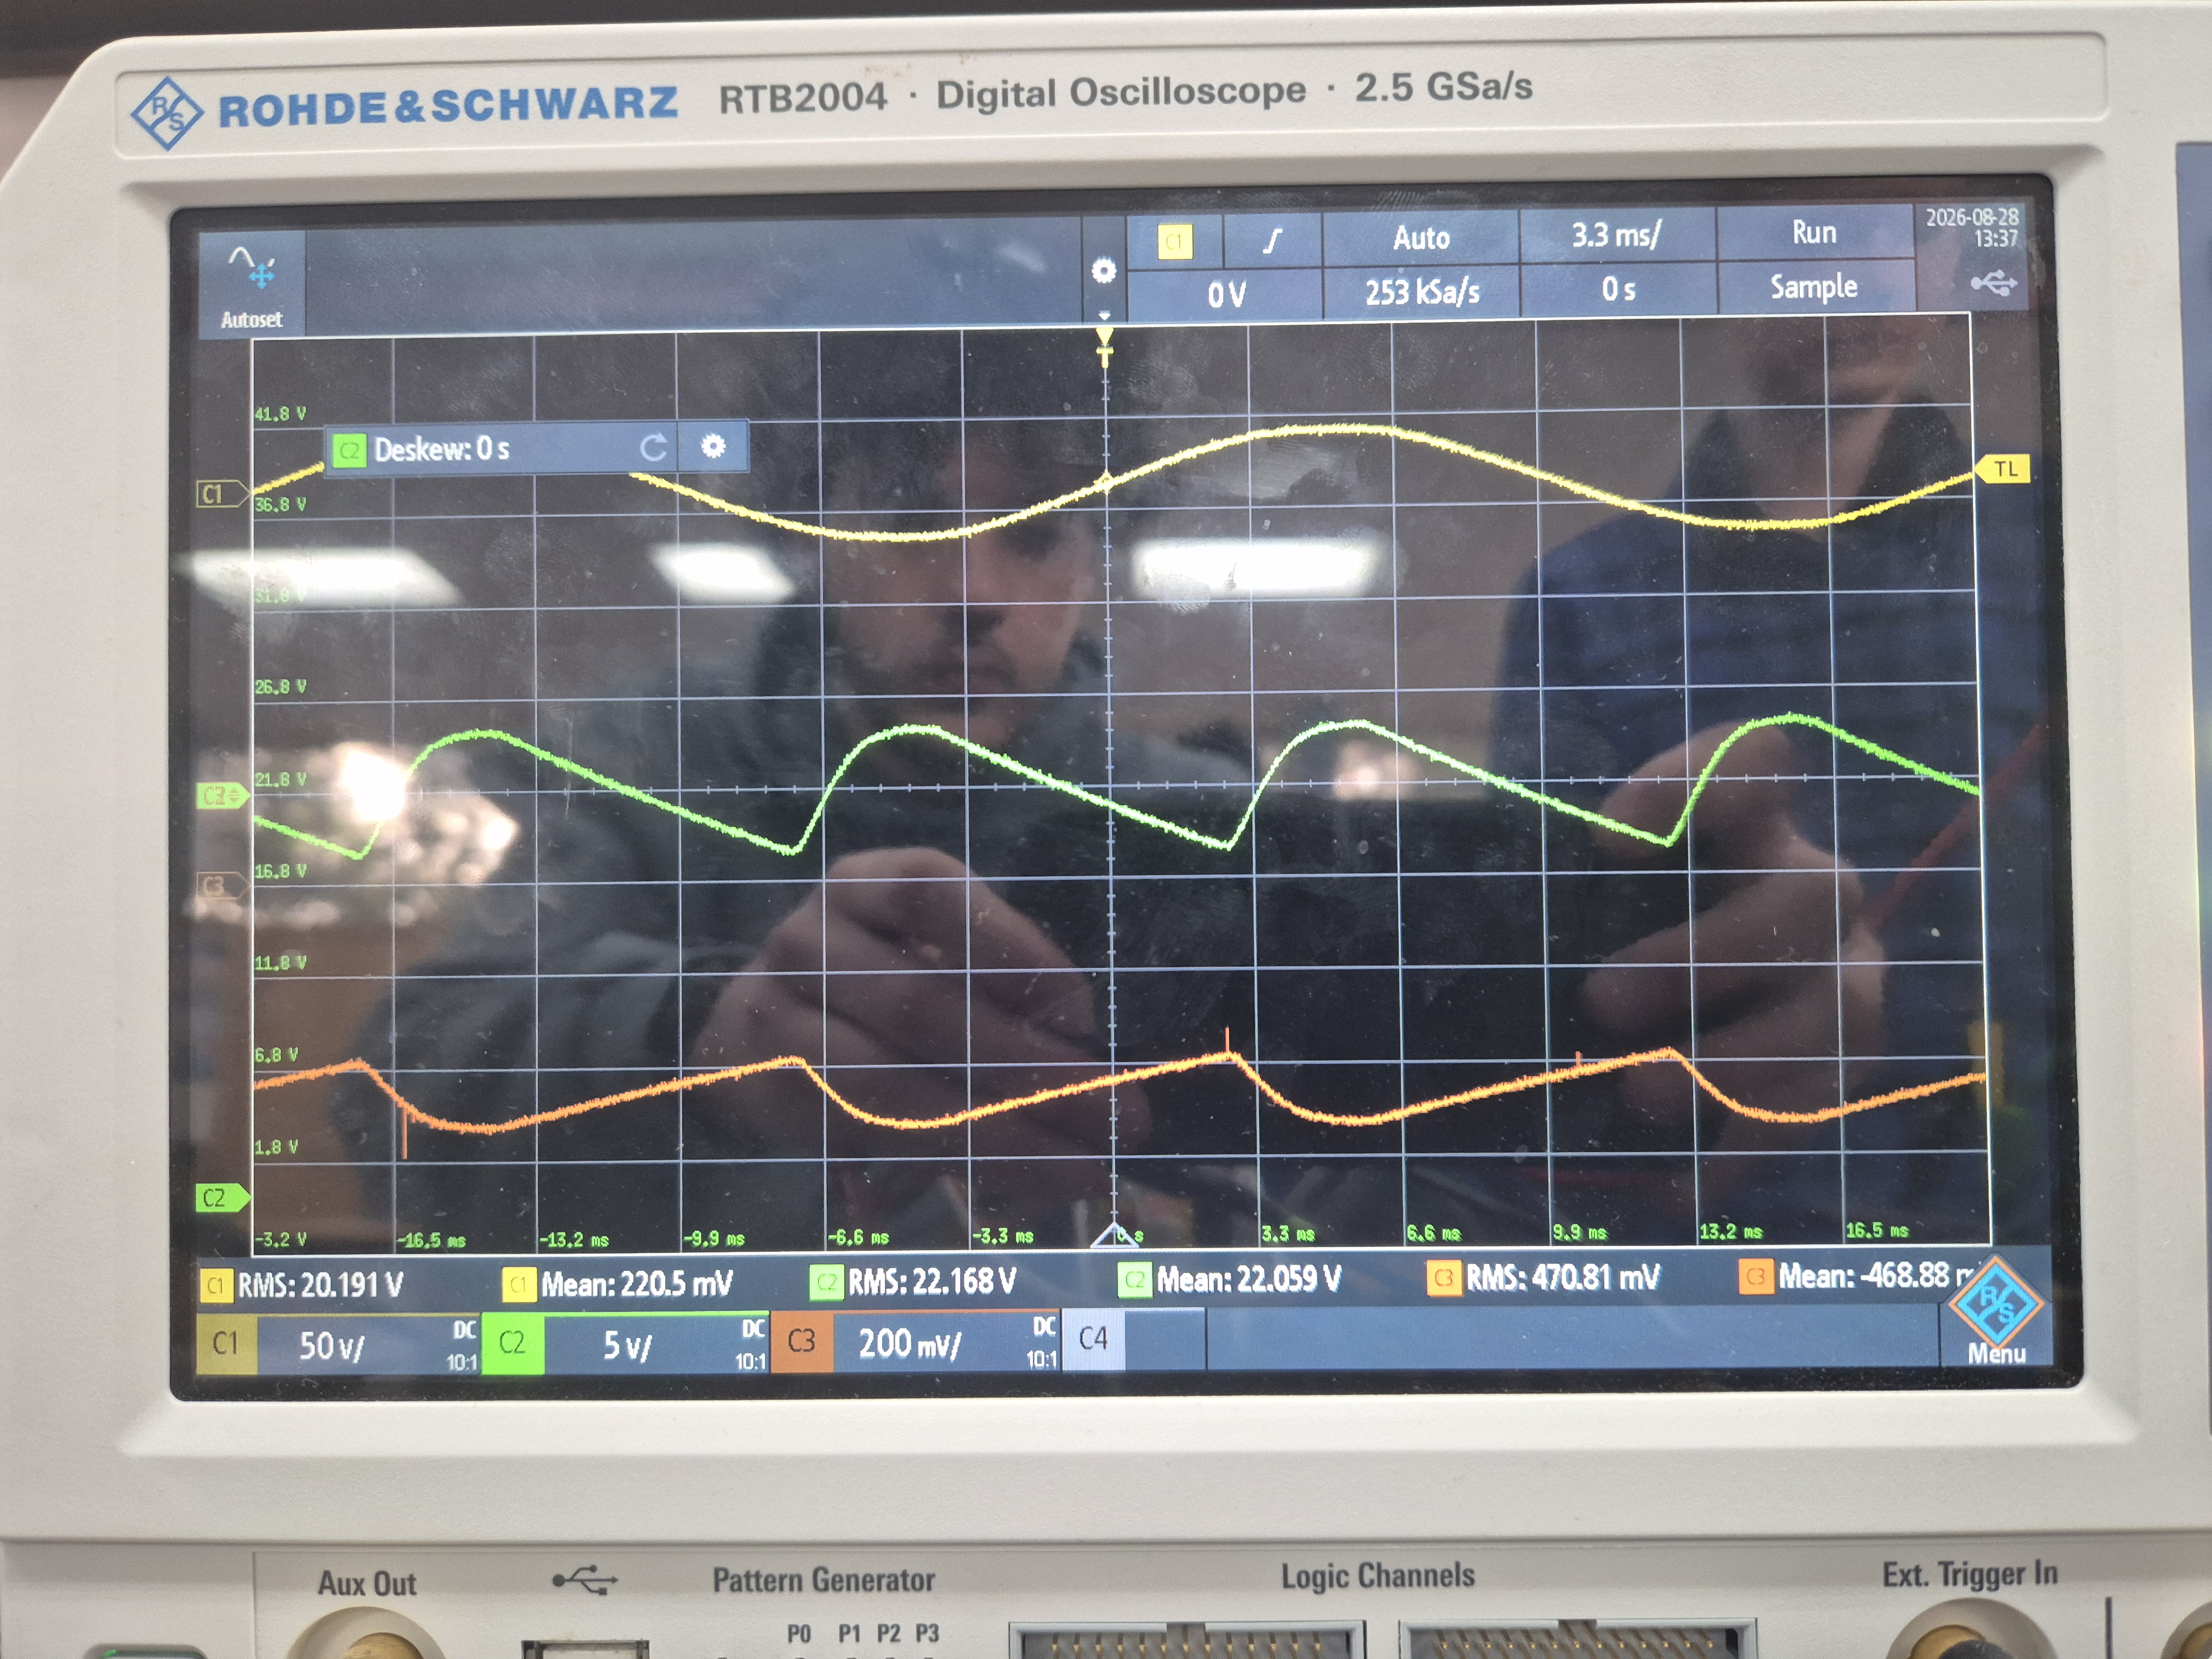
\includegraphics[width=0.7\columnwidth]{Images/20250828_134829.jpg}
	\caption{$470\:F$ Capacitor Plot}
	\label{fig:470F Cap Plot}
\end{figure}
\begin{figure}[H]
        \centering
	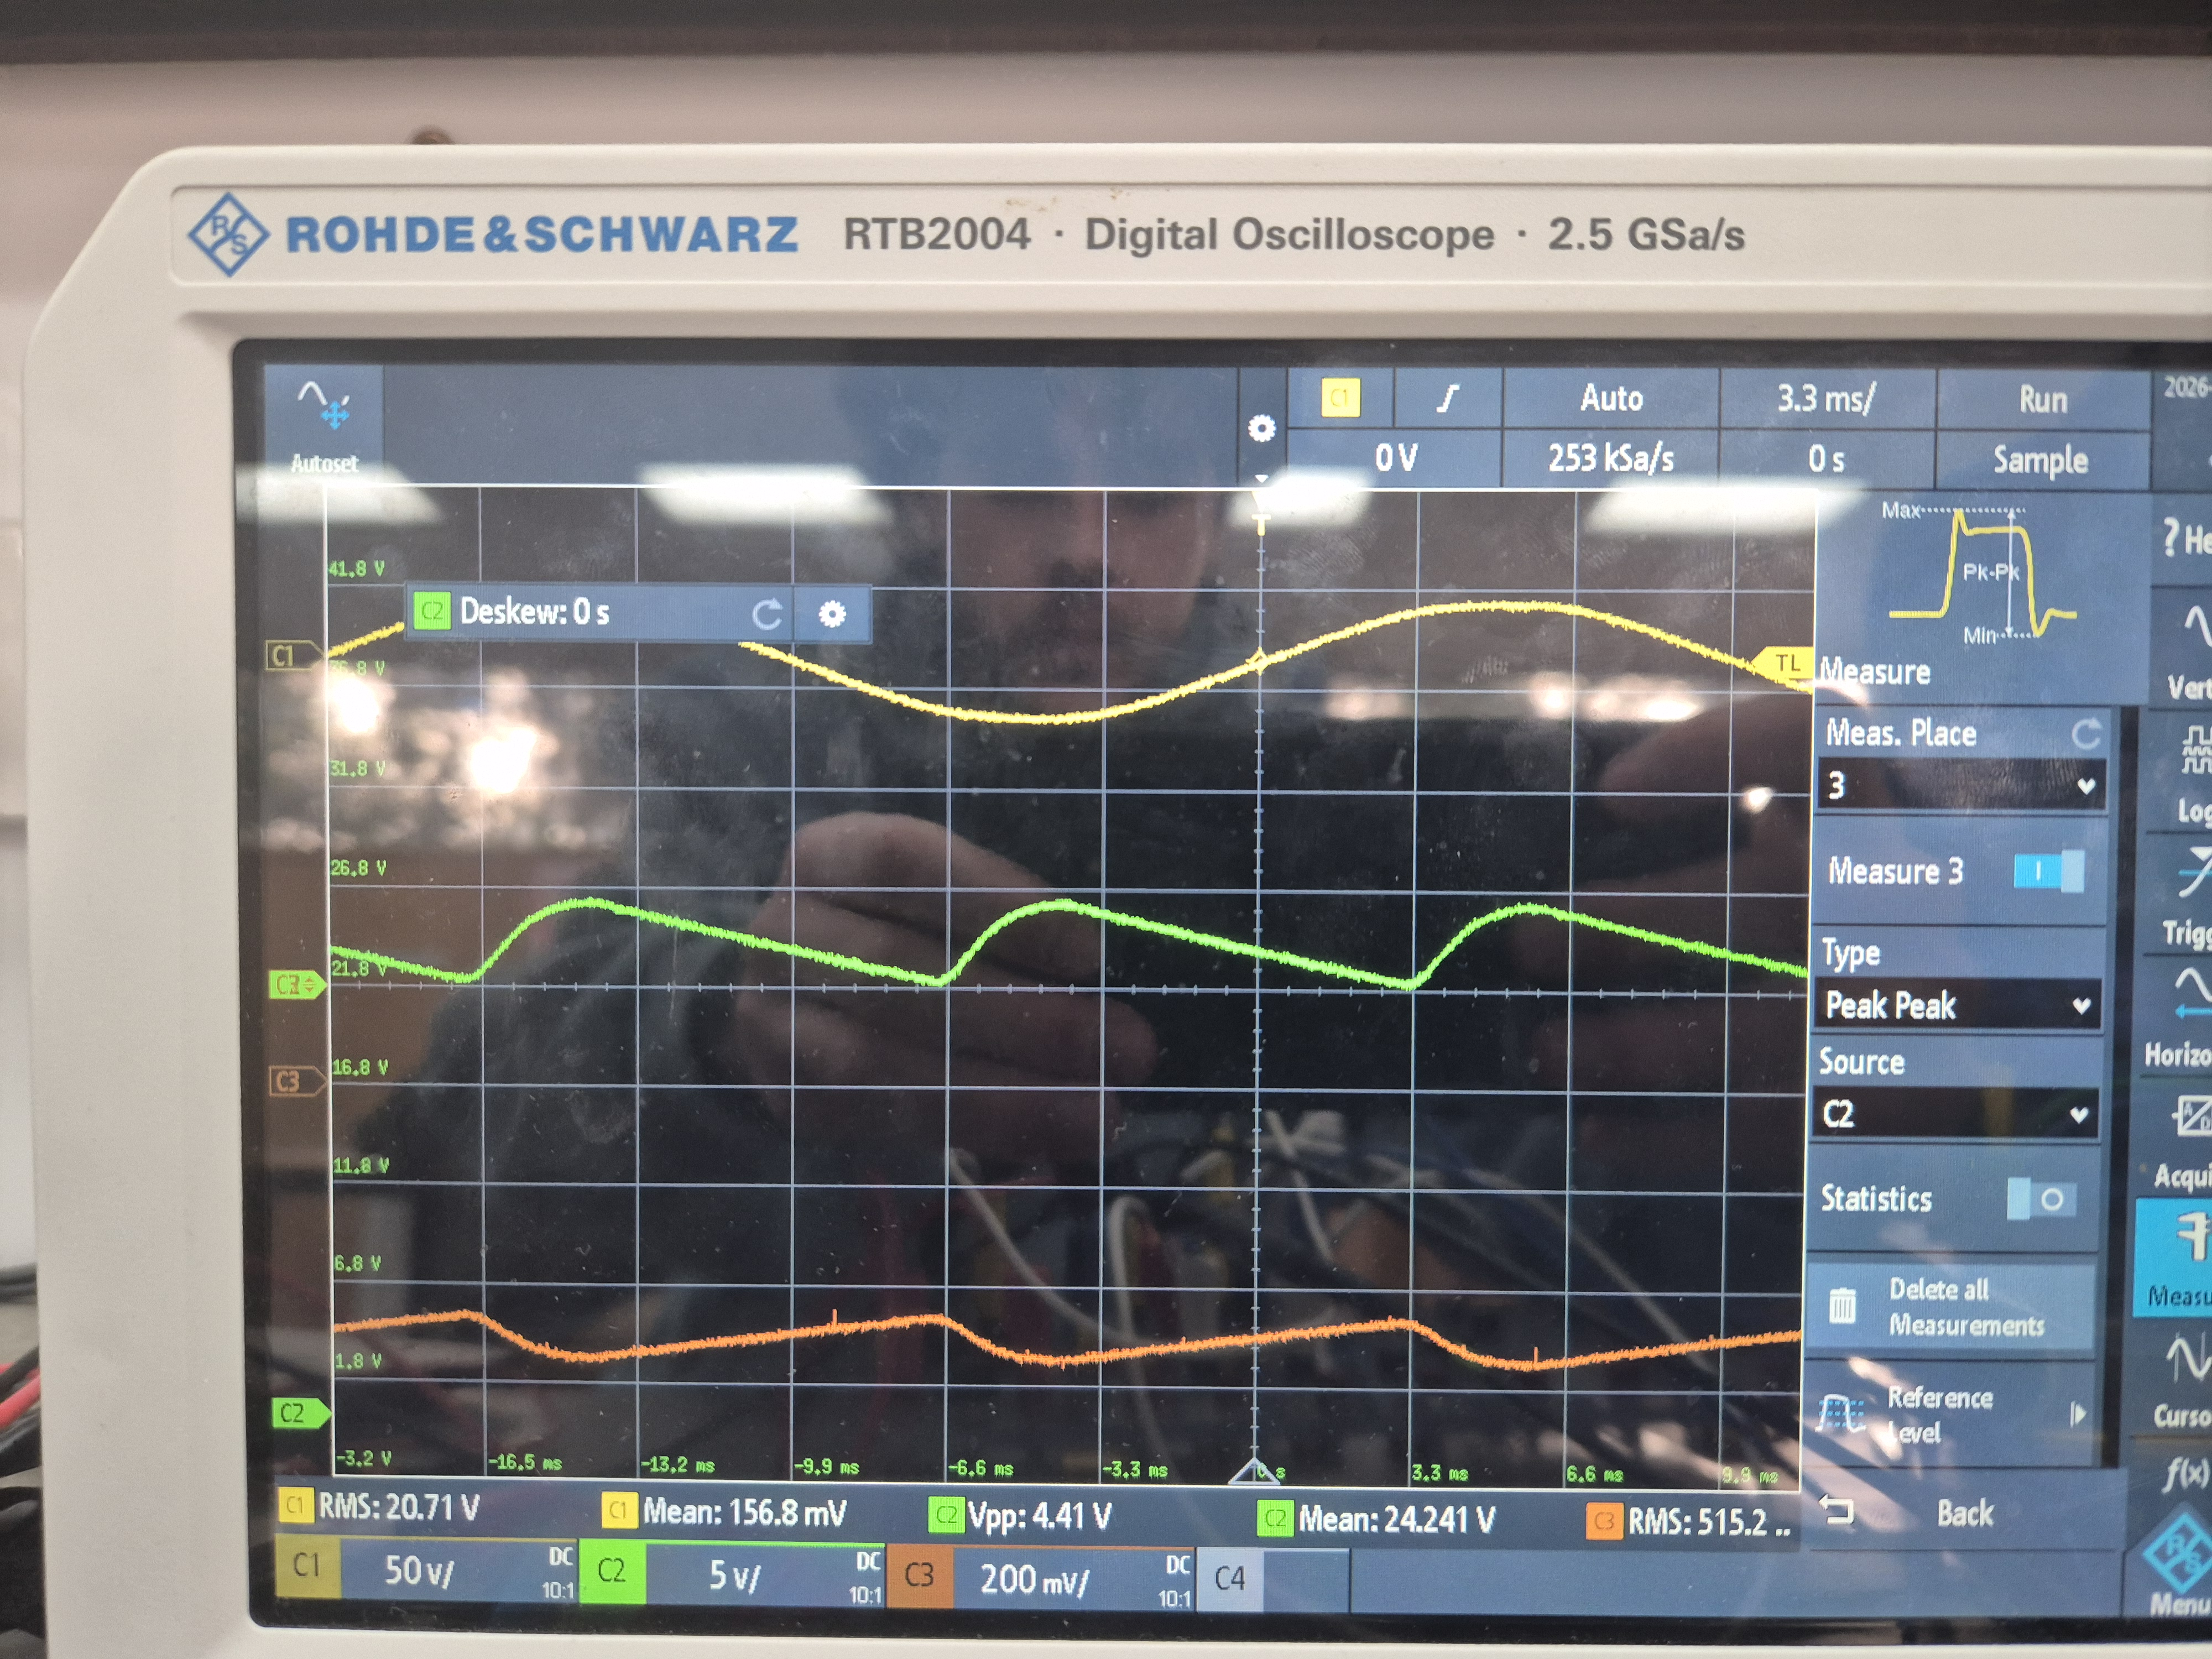
\includegraphics[width=0.7\columnwidth]{Images/20250828_135102.jpg}
	\caption{$1000\:F$ Capacitor Plot}
	\label{fig:1000F Cap Plot}
\end{figure}
\begin{figure}[H]
        \centering
	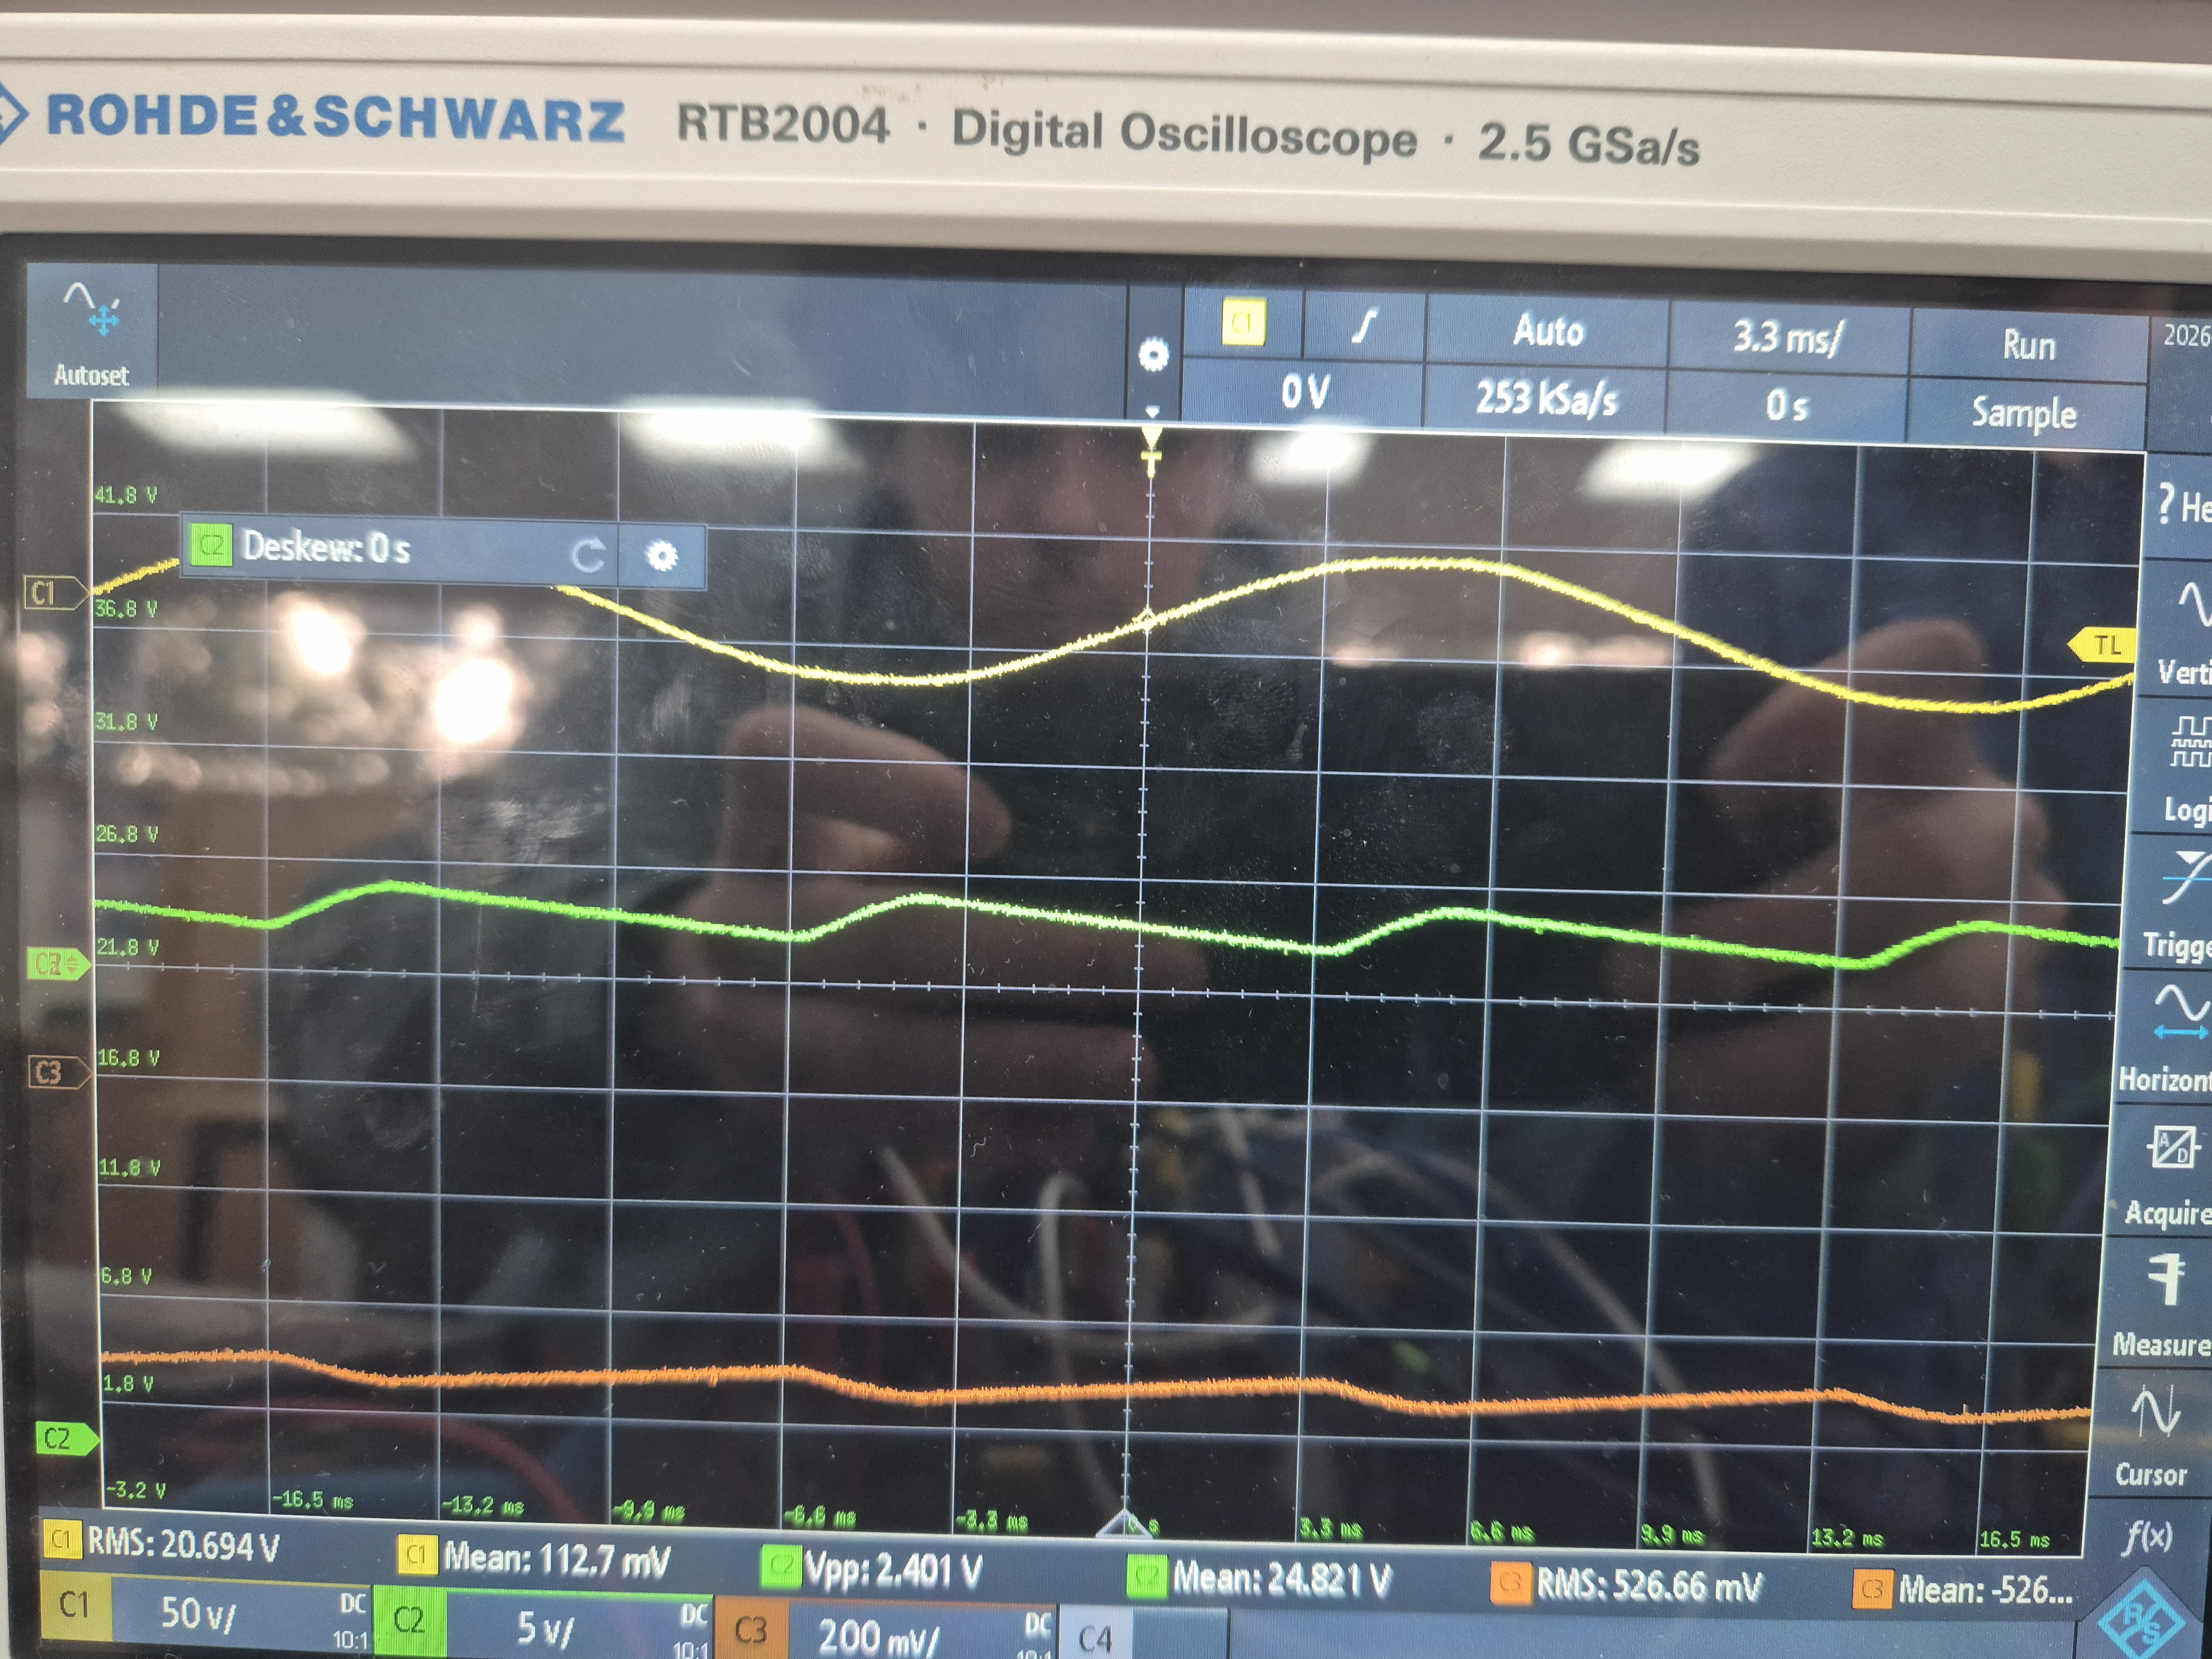
\includegraphics[width=0.7\columnwidth]{Images/20250828_135318.jpg}
	\caption{$2000\:F$ Capacitor Plot}
	\label{fig:2000F Cap Plot}
\end{figure}


\textit{Develop an approximate expression for percentage peak-to-peak ripple as a function of R, C and
frequency $f$, stating carefully any assumptions. How do your calculated values, using your derived
expression, compare to your measurements?}\\

\textit{How would you expect the value of the capacitor to impact upon supply current waveform, in
particular on the harmonic content? Describe why you expect this?
(Note: if you have time you may wish to think of a way to measure and display the Fourier
components of supply current for your circuit, thus gaining extra insight}\\
\section{Thyristor Controller Rectifiers}
\subsection{Semi-Converter with Resistive and Inductive Load}
\begin{center}
\begin{tabular}{|p{3cm}|p{2.5cm}|p{2.5cm}|p{2.5cm}|}
\hline
\centering\textbf{Firing angle} &
\multicolumn{2}{c|}{\textbf{Digital multimeter}} &
\centering\textbf{Calculated} \tabularnewline
\hline
\centering$\alpha$ & \centering$V_o(V)$ & \centering$I_o(mA)$ & \centering$V_o(V)$ \tabularnewline
\hline
0 & 0 & 0 & 0 \\ \hline
20 & 0.8 & 0.8 & 0.384 \\ \hline
45 & 3.4 & 20 & 1.865 \\ \hline
60 & 5.6 & 63 & 3.183 \\ \hline
90 & 9.7 & 159 & 6.366 \\ \hline
100 & 10.2 & 184 & 7.471 \\ \hline
120 & 10.9 & 247 & 9.549 \\ \hline
140 & 10.6 & 285 & 11.243 \\ \hline
160 & 9.5 & 317 & 12.348 \\ \hline
180 & 8.8 & 333 & 12.732 \\ \hline
\end{tabular}
\end{center}\\
To calculate $V_o$ use the formula,
$$V_{o,theory}=K(1-cos(\alpha))$$
where,\\
$$K=\dfrac{V_m}{\pi}=6.366V$$\\
These results can be seen in the table above.\\

\textit{Detail the way you connected your oscilloscope probes and configured the oscilloscope to record simultaneously the source voltage, trigger signal, output voltage and current waveforms.}\\

The common ground is at $+V_o$ to allow for common measurements. Channel 1 measures the source voltage using the secondary transformer winding. This is acceptable as it is electrically isolated from the remainder of the circuit so multiple grounds cannot cause a short circuit. Channel 2 measure the output voltage, with it's positive probe placed at $-V_o$. Channel 3 measures $I_o$, with it's probe placed between the $1\Omega$ and $47\Omega$ resistors. Measuring the voltage over the $1\Omega$ resistor is equivalent to measuring current as $V=IR$. Channel 4 measures the positive trigger input of $T_1$. \\ 

\textit{Include plot from oscilloscope of all waveforms for a firing angle of 45°.}\\

Channel 2 and Channel 3 show the negative output voltage and output current respectively as their ground and positive connections are inverted due to needing a common ground point for all measurements. 
\begin{figure}[H]
        \centering
	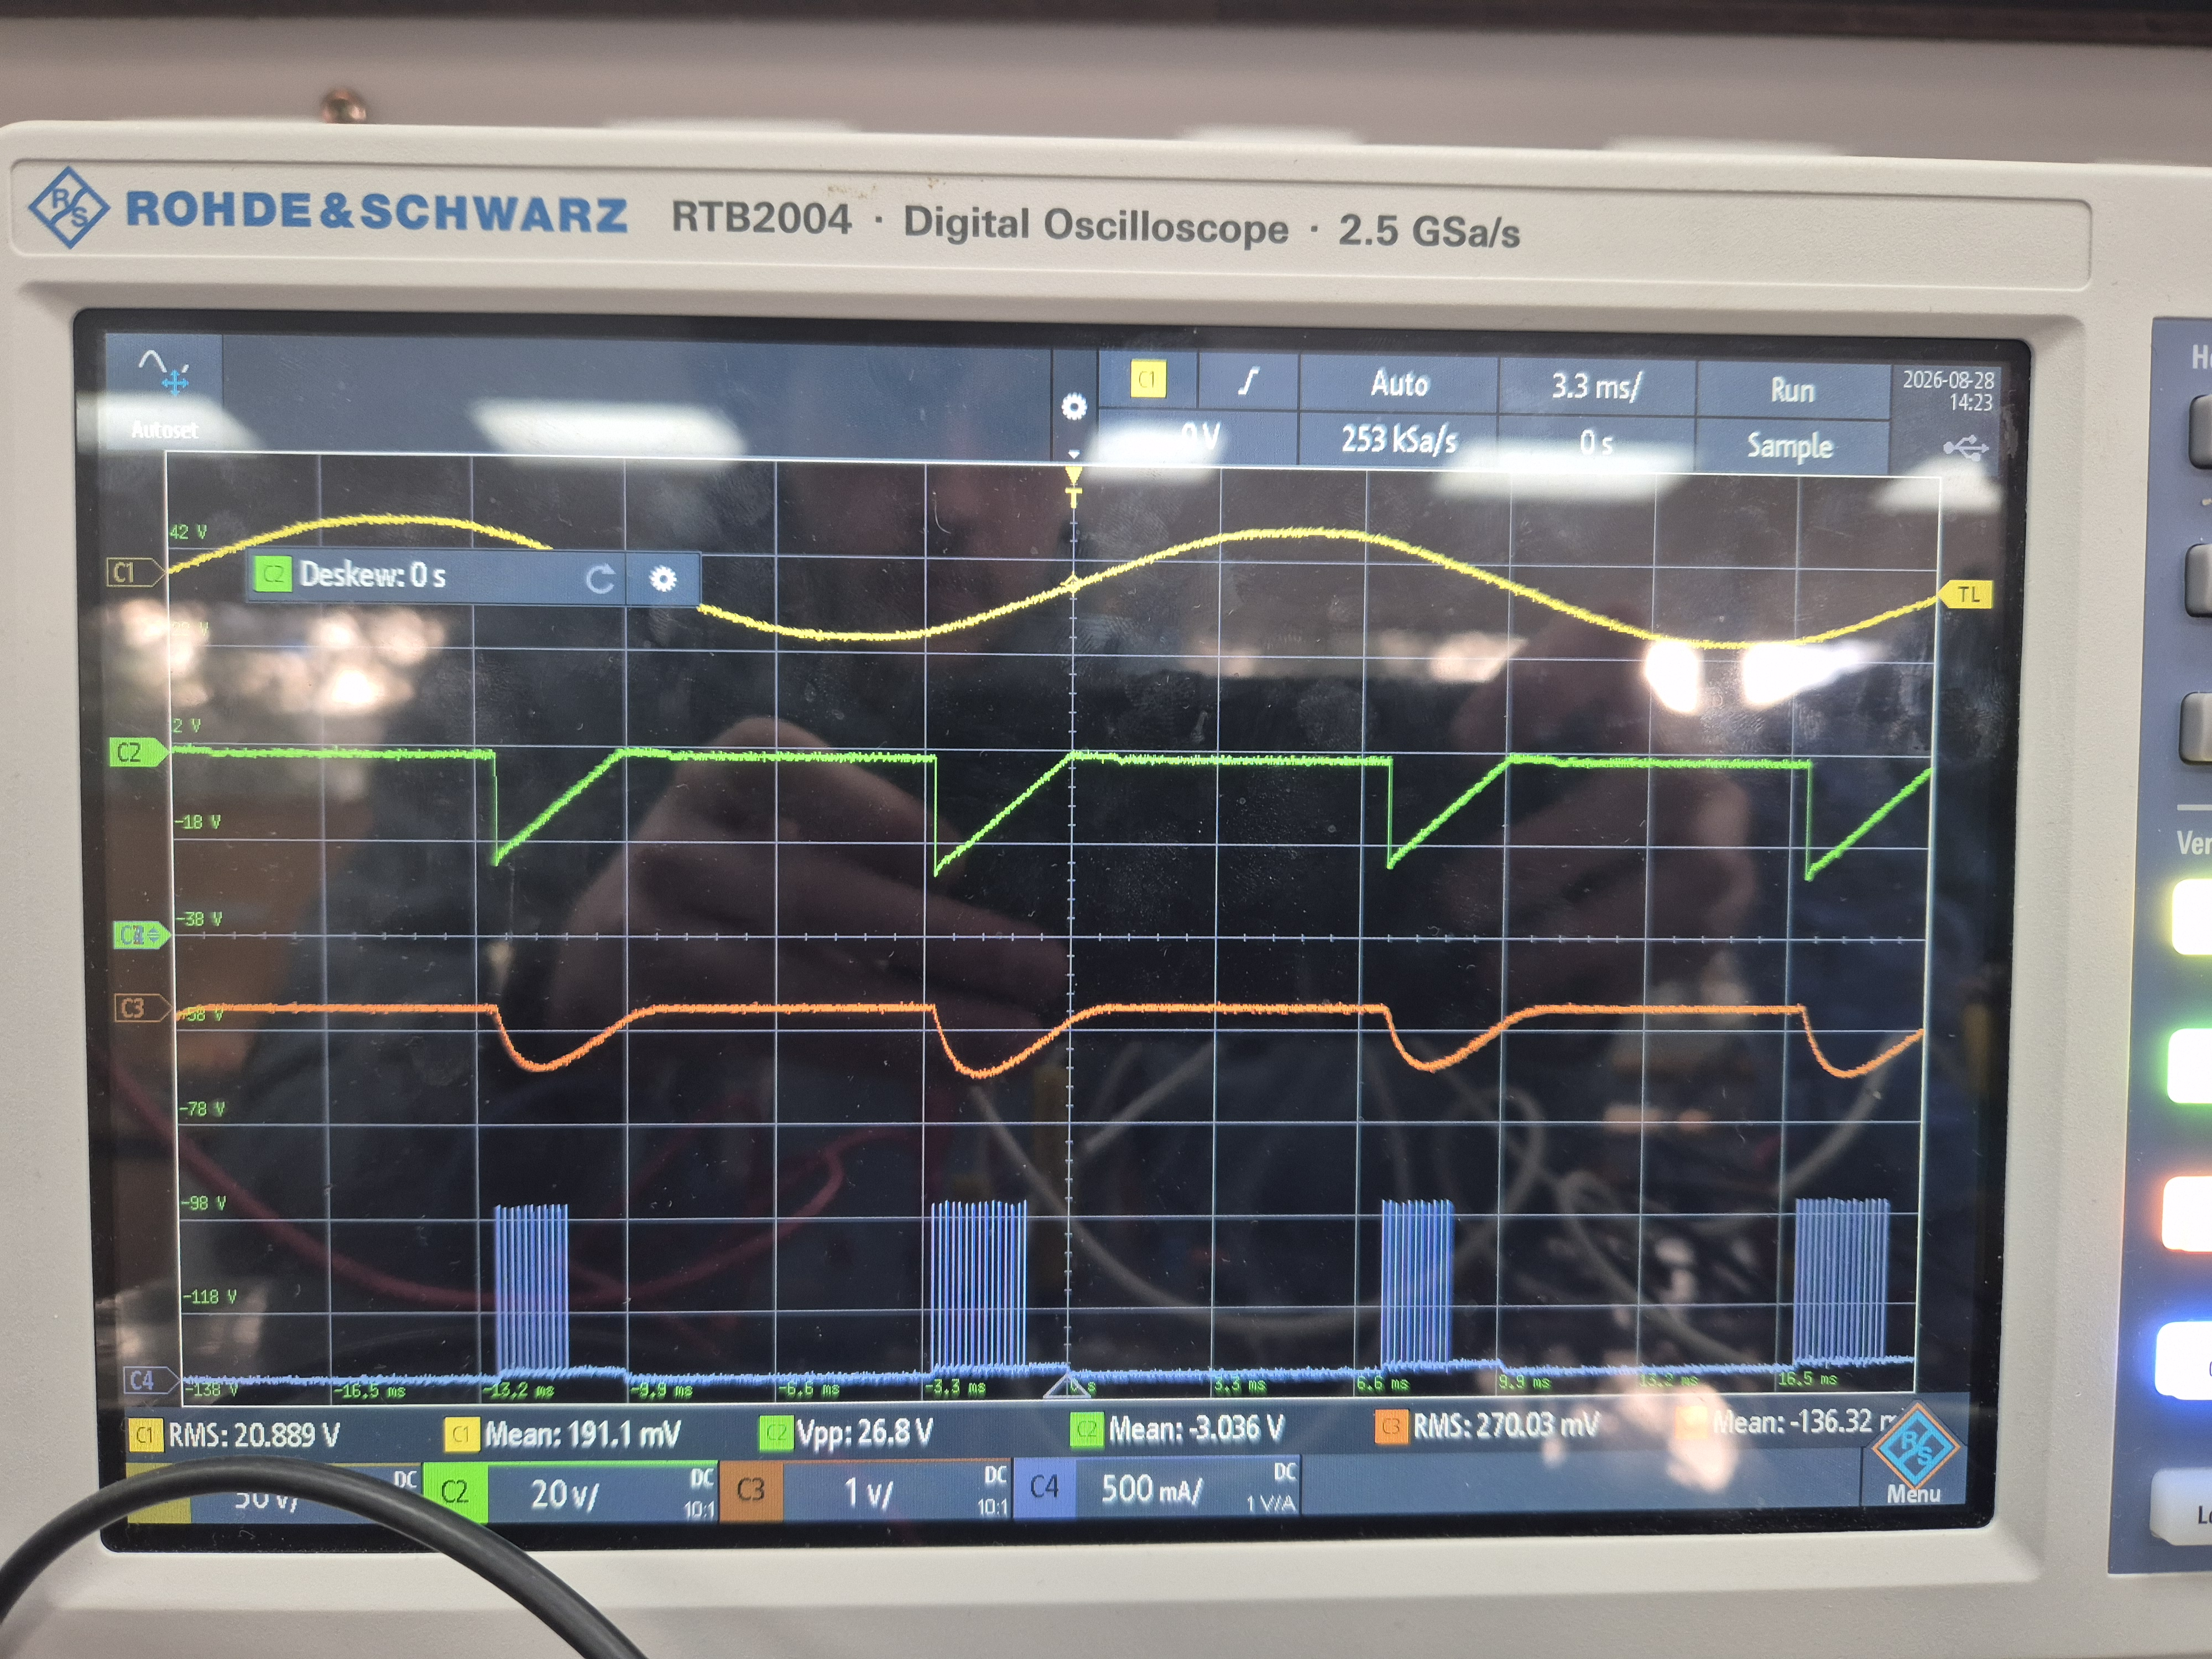
\includegraphics[width=0.7\columnwidth]{Images/20250828_143455.jpg}
	\caption{$45\degree$ firing angle}
	\label{fig:45 degree firing angle}
\end{figure}

\textit{Comment on the observed waveforms and on how they changed with firing angle, describing your observations by considering theory of the circuit operation.}\\

As the firing angle is increased to $180\degree$ the output voltage and current approach the full wave rectified input waveform shown by Channel 1. This is beaus at a firing angle of $180\degree$ the thyristor acts the same as a typical diode used in a full wave rectifier.\\

\textit{From your measured data, create a plot of dc output voltage vs firing angle. Also include in the plot a curve based on theoretical considerations for this circuit. Discuss your findings.}\\

\begin{figure}[H]
        \centering
	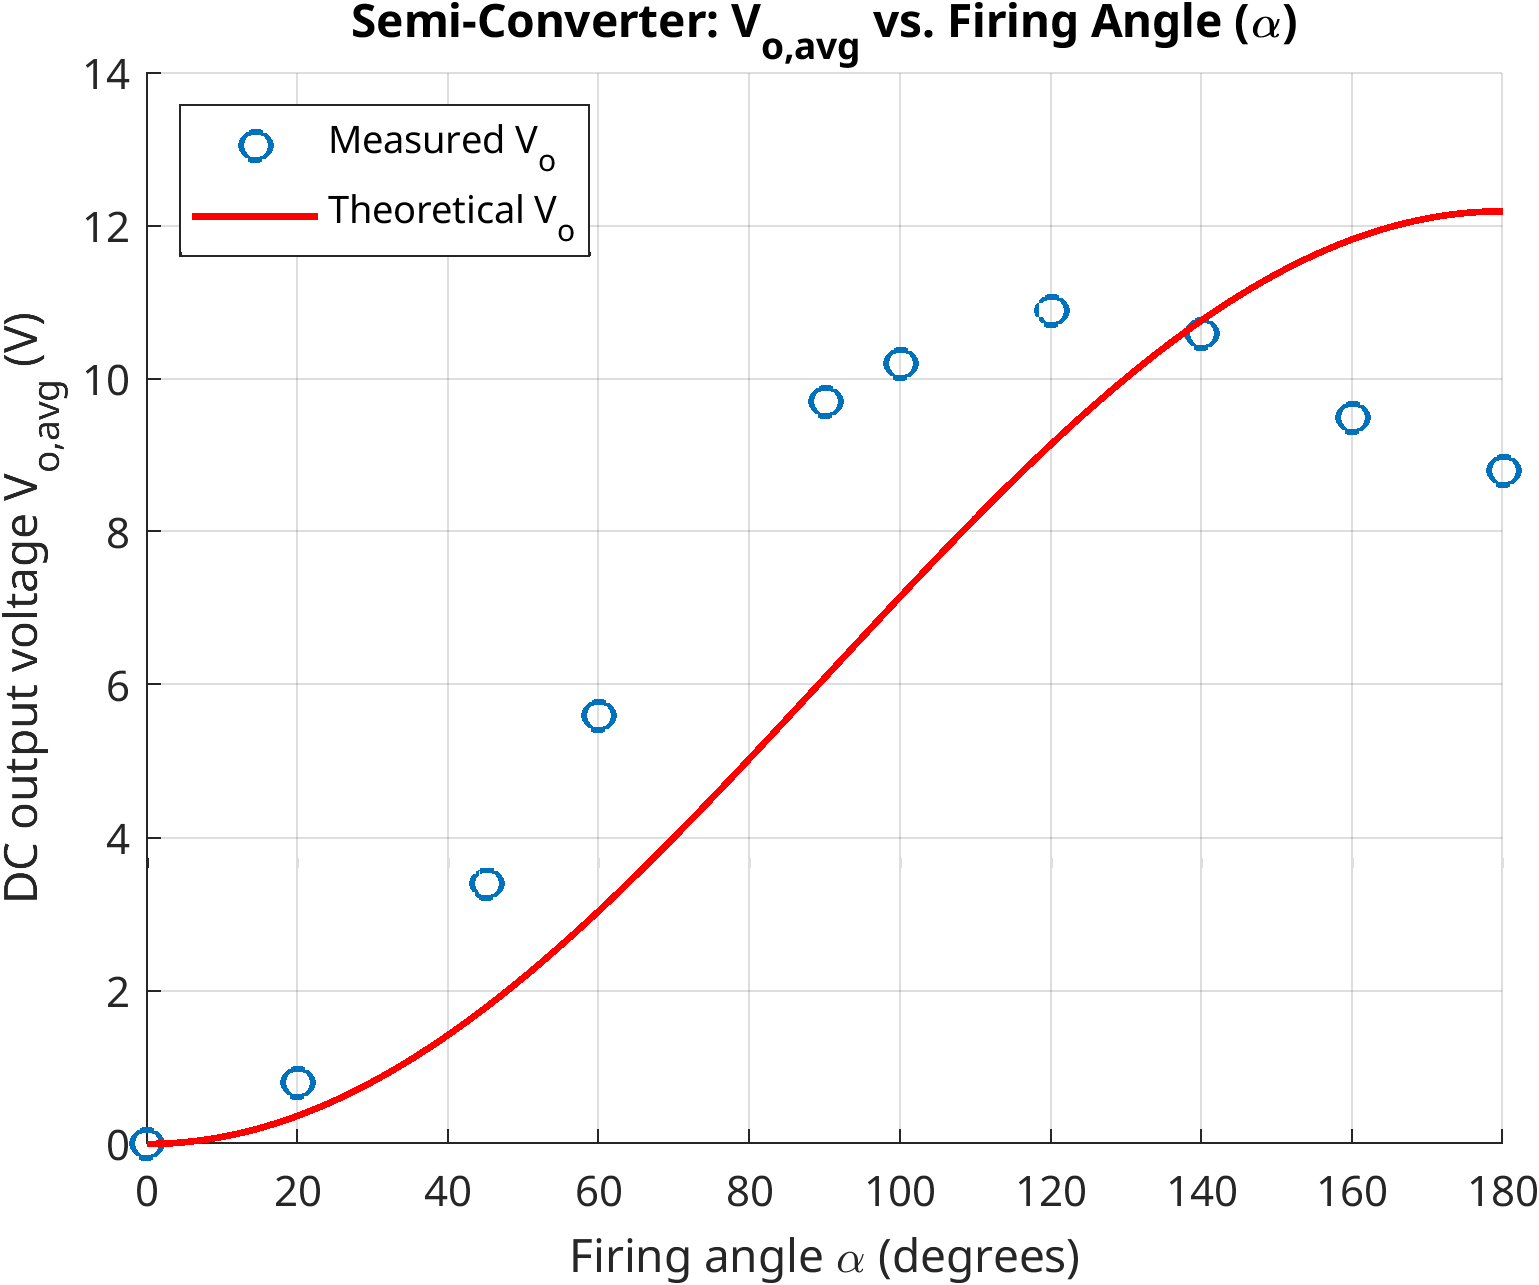
\includegraphics[width=0.7\columnwidth]{Images/semi_converter_correct.png}
	\caption{Output Voltage vs Firing Angle}
	\label{fig:output voltage vs firing angle}
\end{figure}

The theoretical curve $V_{dc}=K(1-\mathrm{cos}\:\alpha)$ matches the measured results with an acceptable error. At a small firing angle the deviations are caused by discontinuous current. The error at higher firing angles may be attributed to residual conduction in the load. There may also be isomer error caused by the non-idealities in the lab configurations.\\

\textit{Based on your observation, at what firing angle did you observe there to first be a boundary between continuous and discontinuous conduction (of current in the load). Compare to what you might expect from a theoretical view point?}\\

The data suggests that the rectifier is is discontinuous conduction mode until approximately $50\degree$ as the average output current is very low suggesting the current drops to zero for parts of the cycle. Above $60\degree$ the output current increases significantly as $\alpha$ increases confirming the current is in continuous conduction mode.\\
Theoretically current should be continuous as long as long as the firing time is long enough for the inductor to store energy to prevent zero current between firing pulses. This means that discontinuous current is expected for low values of $\alpha$ as seen through the measurements.\\

\textit{Describe the purpose of the freewheeling diode in this circuit and what you think might happen if it were removed.}\\

The freewheeling diode provided a safe path for current to flow when the AC input voltage reverse polarity or if the thyristors are turned off. The inductor inherently opposes and sudden current change so a path is required to allow for a gradual decay. This prevents damage to components due to large voltage spikes across the thyristors. It also improves the rectifiers performance by reducing output voltage ripple and smoothing the load current.\\
If the freewheeling diode where to be removed the inductor current would have no alternate discharge paths, leading to discontinuous conduction, higher output ripple and potentially cause damage to the thyristors due to the inductor's stored energy.

\section{Reflection}

TODO: 

\vfill
\hrule
\begin{center}
\textit{End of Report}
\end{center}
\end{document}
